\documentclass{article}

% if you need to pass options to natbib, use, e.g.:
% \PassOptionsToPackage{numbers, compress}{natbib}
% before loading nips_2017
%
% to avoid loading the natbib package, add option nonatbib:
%\usepackage[nonatbib]{nips_2017}

\usepackage{nips_2017}

% to compile a camera-ready version, add the [final] option, e.g.:
% \usepackage[final]{nips_2017}

\usepackage[utf8]{inputenc} % allow utf-8 input
\usepackage[T1]{fontenc}    % use 8-bit T1 fonts
\usepackage{hyperref}       % hyperlinks
\usepackage{url}            % simple URL typesetting
\usepackage{booktabs}       % professional-quality tables
\usepackage{amsfonts}       % blackboard math symbols
\usepackage{nicefrac}       % compact symbols for 1/2, etc.
\usepackage{microtype}      % microtypography
\usepackage{tikz,placeins}
\usepackage{subcaption}
%\usepackage[caption = false]{subfig}
\usepackage{amssymb,amsmath,bm}
\usetikzlibrary{arrows,decorations.markings}
\tikzstyle{every picture}+=[font=\rmfamily\it\bfseries\large]

\graphicspath{{../figures/}}

\title{A state of the art end-to-end speech recognition algorithm with
a homogenous structure.}

%\renewcommand{\vec}[1]{\mathbf{#1}}

\newcommand{\chanwcom}{{C. Kim}}
\renewcommand{\topfraction}{0.85}
\renewcommand{\textfraction}{0.1}
\renewcommand{\floatpagefraction}{0.85}

% The \author macro works with any number of authors. There are two
% commands used to separate the names and addresses of multiple
% authors: \And and \AND.
%
% Using \And between authors leaves it to LaTeX to determine where to
% break the lines. Using \AND forces a line break at that point. So,
% if LaTeX puts 3 of 4 authors names on the first line, and the last
% on the second line, try using \AND instead of \And before the third
% author name.

\author{
  David S.~Hippocampus\thanks{Use footnote for providing further
    information about author (webpage, alternative
    address)---\emph{not} for acknowledging funding agencies.} \\
  Department of Computer Science\\
  Cranberry-Lemon University\\
  Pittsburgh, PA 15213 \\
  \texttt{hippo@cs.cranberry-lemon.edu} \\
  %% examples of more authors
  %% \And
  %% Coauthor \\
  %% Affiliation \\
  %% Address \\
  %% \texttt{email} \\
  %% \AND
  %% Coauthor \\
  %% Affiliation \\
  %% Address \\
  %% \texttt{email} \\
  %% \And
  %% Coauthor \\
  %% Affiliation \\
  %% Address \\
  %% \texttt{email} \\
  %% \And
  %% Coauthor \\
  %% Affiliation \\
  %% Address \\
  %% \texttt{email} \\
}

\begin{document}
% \nipsfinalcopy is no longer used

\maketitle

\begin{abstract}
TODO(chanw.com) Revise the abstract.
This paper proposes a new end-to-end speech recognition system referred to
as Recurrent neural network Sequence Classification (RSC). Recently, end-to-end speech
recognition systems have been gaining more attention from researchers and
several different structures have been proposed. Typical examples  
include Connectionist Temporal Classification (CTC), Recurrent Neural Network
  Transducer (RNN-T), and Sequence-to-Sequence Modeling using the attention
mechanism. The CTC-based approaches are using the CTC loss assuming the
conditional independence property. Although the structure of CTC is simpler
than other end-to-end systems, the performance is worse due to this conditional
independence assumption. RNN-T and attention-based approaches have distinct
components such as the prediction network  and encoder in RNN-T, and
the encoder, the decoder, and the attention layer in the attention-based model.
Compared to these models, SHC has a homogeneous structure from the bottom to 
the top layer. LSTM and max-pooling layer are repeated followed by the top
softmax layer. The embedded softmax output is fed back as input of each RNN
layer. The training starts with flat initialization and alignment is made
after every epoch. The loss is the Cross Entropy (CE) loss using this 
alignment result. In our experimental results, SHC algorithm has shown 
better performance than more complicated attention-based end-to-end speech
recognition system. Another major advantage is training is significantly
faster.
\end{abstract}

\section{Introduction}

Recently, deep neural network has significantly improved the performance
of speech recognition systems \cite{}.


\section{Review of end-to-end speech recognition systems}

\begin{figure}
    \centering
    \resizebox{40mm}{!}{%
         % Graphic for TeX using PGF
% Title: /home/chanwcom/chanwcom_local_repository/experimental/my_papers/papers_working/icml_2018_monolitic_end_to_end/figures/ctc.dia
% Creator: Dia v0.97.3
% CreationDate: Tue Jan 22 18:35:52 2019
% For: chanwcom
% \usepackage{tikz}
% The following commands are not supported in PSTricks at present
% We define them conditionally, so when they are implemented,
% this pgf file will use them.
\ifx\du\undefined
  \newlength{\du}
\fi
\setlength{\du}{15\unitlength}
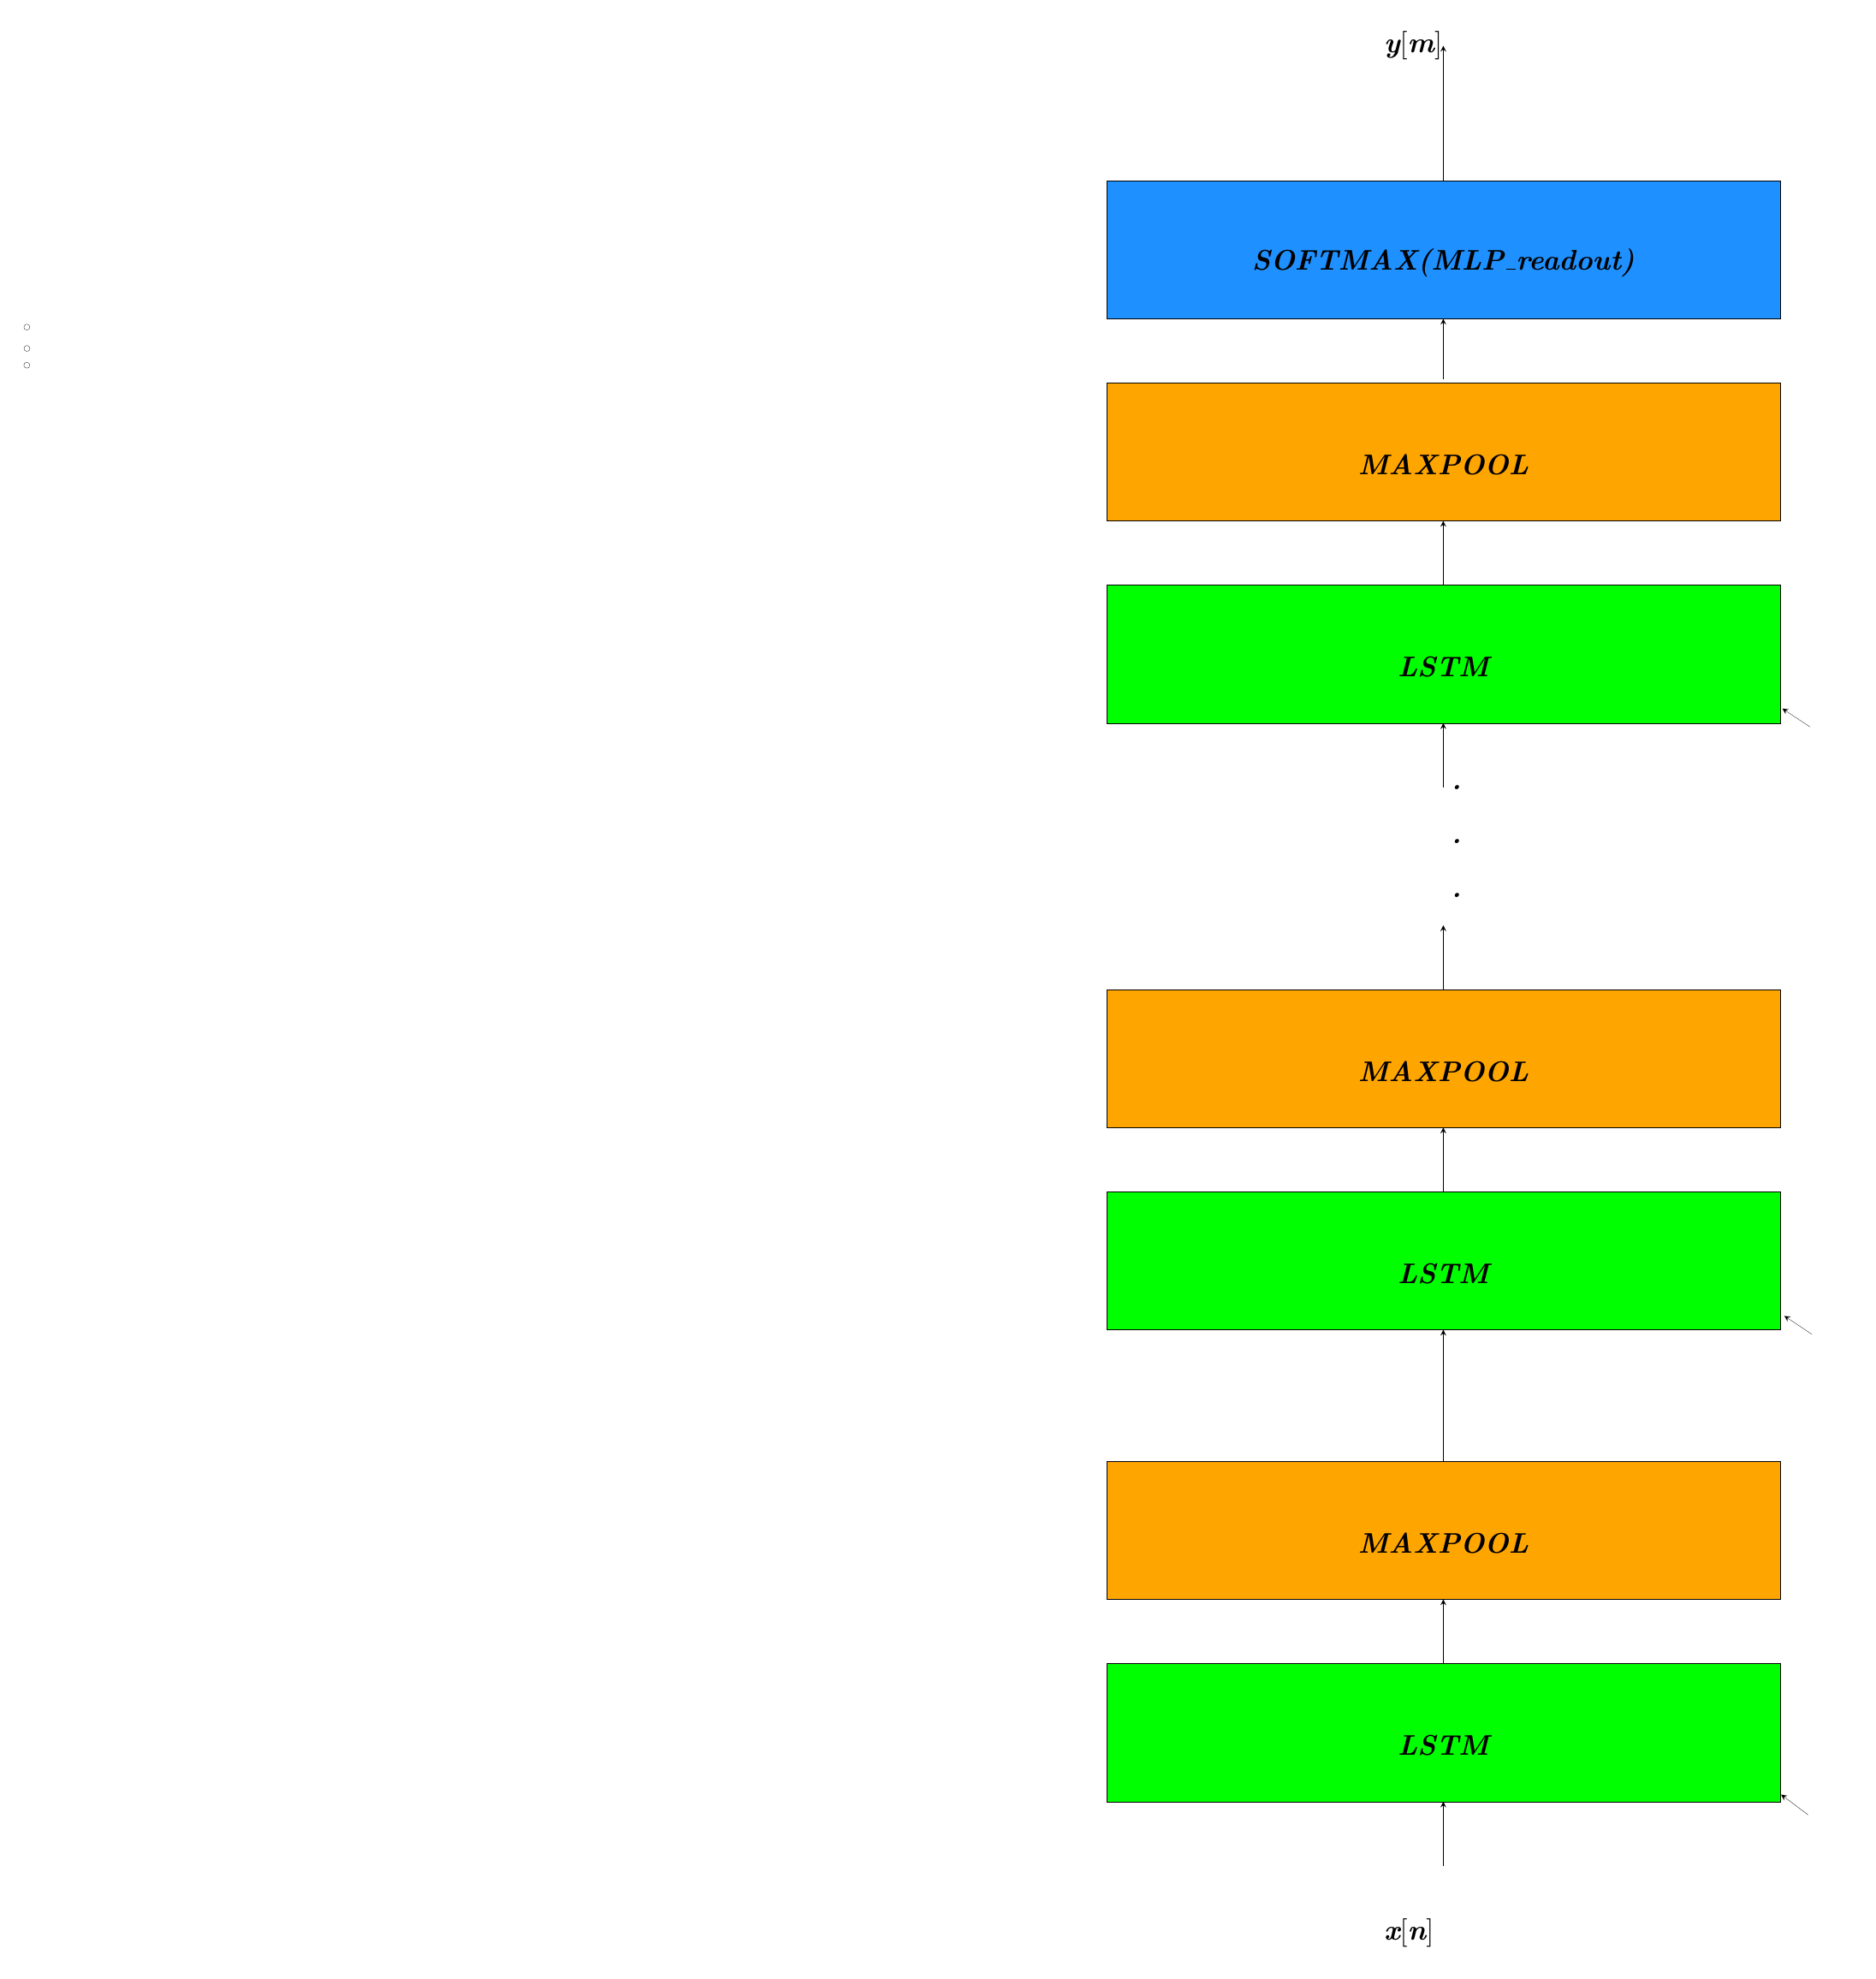
\begin{tikzpicture}
\pgftransformxscale{1.000000}
\pgftransformyscale{-1.000000}
\definecolor{dialinecolor}{rgb}{0.000000, 0.000000, 0.000000}
\pgfsetstrokecolor{dialinecolor}
\definecolor{dialinecolor}{rgb}{1.000000, 1.000000, 1.000000}
\pgfsetfillcolor{dialinecolor}
\definecolor{dialinecolor}{rgb}{1.000000, 1.000000, 1.000000}
\pgfsetfillcolor{dialinecolor}
\pgfpathellipse{\pgfpoint{27.921843\du}{4.950110\du}}{\pgfpoint{1.258243\du}{0\du}}{\pgfpoint{0\du}{1.250000\du}}
\pgfusepath{fill}
\pgfsetlinewidth{0.100000\du}
\pgfsetdash{}{0pt}
\pgfsetdash{}{0pt}
\pgfsetmiterjoin
\definecolor{dialinecolor}{rgb}{0.000000, 0.000000, 0.000000}
\pgfsetstrokecolor{dialinecolor}
\pgfpathellipse{\pgfpoint{27.921843\du}{4.950110\du}}{\pgfpoint{1.258243\du}{0\du}}{\pgfpoint{0\du}{1.250000\du}}
\pgfusepath{stroke}
% setfont left to latex
\definecolor{dialinecolor}{rgb}{0.000000, 0.000000, 0.000000}
\pgfsetstrokecolor{dialinecolor}
\node at (27.921843\du,5.145110\du){};
\definecolor{dialinecolor}{rgb}{1.000000, 1.000000, 1.000000}
\pgfsetfillcolor{dialinecolor}
\pgfpathellipse{\pgfpoint{27.949843\du}{13.960800\du}}{\pgfpoint{1.258243\du}{0\du}}{\pgfpoint{0\du}{1.250000\du}}
\pgfusepath{fill}
\pgfsetlinewidth{0.100000\du}
\pgfsetdash{}{0pt}
\pgfsetdash{}{0pt}
\pgfsetmiterjoin
\definecolor{dialinecolor}{rgb}{0.000000, 0.000000, 0.000000}
\pgfsetstrokecolor{dialinecolor}
\pgfpathellipse{\pgfpoint{27.949843\du}{13.960800\du}}{\pgfpoint{1.258243\du}{0\du}}{\pgfpoint{0\du}{1.250000\du}}
\pgfusepath{stroke}
% setfont left to latex
\definecolor{dialinecolor}{rgb}{0.000000, 0.000000, 0.000000}
\pgfsetstrokecolor{dialinecolor}
\node at (27.949843\du,14.155800\du){};
\definecolor{dialinecolor}{rgb}{1.000000, 0.647059, 0.000000}
\pgfsetfillcolor{dialinecolor}
\fill (17.000000\du,17.000000\du)--(17.000000\du,19.050000\du)--(27.000000\du,19.050000\du)--(27.000000\du,17.000000\du)--cycle;
\pgfsetlinewidth{0.100000\du}
\pgfsetdash{}{0pt}
\pgfsetdash{}{0pt}
\pgfsetmiterjoin
\definecolor{dialinecolor}{rgb}{0.000000, 0.000000, 0.000000}
\pgfsetstrokecolor{dialinecolor}
\draw (17.000000\du,17.000000\du)--(17.000000\du,19.050000\du)--(27.000000\du,19.050000\du)--(27.000000\du,17.000000\du)--cycle;
% setfont left to latex
\definecolor{dialinecolor}{rgb}{0.000000, 0.000000, 0.000000}
\pgfsetstrokecolor{dialinecolor}
\node at (22.000000\du,18.220000\du){MAXPOOL};
\definecolor{dialinecolor}{rgb}{0.000000, 1.000000, 0.000000}
\pgfsetfillcolor{dialinecolor}
\fill (17.000000\du,4.000000\du)--(17.000000\du,6.050000\du)--(27.000000\du,6.050000\du)--(27.000000\du,4.000000\du)--cycle;
\pgfsetlinewidth{0.100000\du}
\pgfsetdash{}{0pt}
\pgfsetdash{}{0pt}
\pgfsetmiterjoin
\definecolor{dialinecolor}{rgb}{0.000000, 0.000000, 0.000000}
\pgfsetstrokecolor{dialinecolor}
\draw (17.000000\du,4.000000\du)--(17.000000\du,6.050000\du)--(27.000000\du,6.050000\du)--(27.000000\du,4.000000\du)--cycle;
% setfont left to latex
\definecolor{dialinecolor}{rgb}{0.000000, 0.000000, 0.000000}
\pgfsetstrokecolor{dialinecolor}
\node at (22.000000\du,5.220000\du){LSTM};
\definecolor{dialinecolor}{rgb}{0.000000, 1.000000, 0.000000}
\pgfsetfillcolor{dialinecolor}
\fill (17.000000\du,13.000000\du)--(17.000000\du,15.050000\du)--(27.000000\du,15.050000\du)--(27.000000\du,13.000000\du)--cycle;
\pgfsetlinewidth{0.100000\du}
\pgfsetdash{}{0pt}
\pgfsetdash{}{0pt}
\pgfsetmiterjoin
\definecolor{dialinecolor}{rgb}{0.000000, 0.000000, 0.000000}
\pgfsetstrokecolor{dialinecolor}
\draw (17.000000\du,13.000000\du)--(17.000000\du,15.050000\du)--(27.000000\du,15.050000\du)--(27.000000\du,13.000000\du)--cycle;
% setfont left to latex
\definecolor{dialinecolor}{rgb}{0.000000, 0.000000, 0.000000}
\pgfsetstrokecolor{dialinecolor}
\node at (22.000000\du,14.220000\du){LSTM};
\definecolor{dialinecolor}{rgb}{1.000000, 0.647059, 0.000000}
\pgfsetfillcolor{dialinecolor}
\fill (17.000000\du,10.000000\du)--(17.000000\du,12.050000\du)--(27.000000\du,12.050000\du)--(27.000000\du,10.000000\du)--cycle;
\pgfsetlinewidth{0.100000\du}
\pgfsetdash{}{0pt}
\pgfsetdash{}{0pt}
\pgfsetmiterjoin
\definecolor{dialinecolor}{rgb}{0.000000, 0.000000, 0.000000}
\pgfsetstrokecolor{dialinecolor}
\draw (17.000000\du,10.000000\du)--(17.000000\du,12.050000\du)--(27.000000\du,12.050000\du)--(27.000000\du,10.000000\du)--cycle;
% setfont left to latex
\definecolor{dialinecolor}{rgb}{0.000000, 0.000000, 0.000000}
\pgfsetstrokecolor{dialinecolor}
\node at (22.000000\du,11.220000\du){MAXPOOL};
\definecolor{dialinecolor}{rgb}{0.117647, 0.564706, 1.000000}
\pgfsetfillcolor{dialinecolor}
\fill (17.000000\du,-2.000000\du)--(17.000000\du,0.050000\du)--(27.000000\du,0.050000\du)--(27.000000\du,-2.000000\du)--cycle;
\pgfsetlinewidth{0.100000\du}
\pgfsetdash{}{0pt}
\pgfsetdash{}{0pt}
\pgfsetmiterjoin
\definecolor{dialinecolor}{rgb}{0.000000, 0.000000, 0.000000}
\pgfsetstrokecolor{dialinecolor}
\draw (17.000000\du,-2.000000\du)--(17.000000\du,0.050000\du)--(27.000000\du,0.050000\du)--(27.000000\du,-2.000000\du)--cycle;
% setfont left to latex
\definecolor{dialinecolor}{rgb}{0.000000, 0.000000, 0.000000}
\pgfsetstrokecolor{dialinecolor}
\node at (22.000000\du,-0.780000\du){SOFTMAX(MLP\_readout)};
\pgfsetlinewidth{0.100000\du}
\pgfsetdash{}{0pt}
\pgfsetdash{}{0pt}
\pgfsetbuttcap
{
\definecolor{dialinecolor}{rgb}{0.000000, 0.000000, 0.000000}
\pgfsetfillcolor{dialinecolor}
% was here!!!
\pgfsetarrowsend{stealth}
\definecolor{dialinecolor}{rgb}{0.000000, 0.000000, 0.000000}
\pgfsetstrokecolor{dialinecolor}
\draw (22.000000\du,23.000000\du)--(22.000000\du,22.050000\du);
}
\pgfsetlinewidth{0.100000\du}
\pgfsetdash{}{0pt}
\pgfsetdash{}{0pt}
\pgfsetbuttcap
{
\definecolor{dialinecolor}{rgb}{0.000000, 0.000000, 0.000000}
\pgfsetfillcolor{dialinecolor}
% was here!!!
\pgfsetarrowsend{stealth}
\definecolor{dialinecolor}{rgb}{0.000000, 0.000000, 0.000000}
\pgfsetstrokecolor{dialinecolor}
\draw (22.000000\du,20.000000\du)--(22.000000\du,19.050000\du);
}
\pgfsetlinewidth{0.100000\du}
\pgfsetdash{}{0pt}
\pgfsetdash{}{0pt}
\pgfsetbuttcap
{
\definecolor{dialinecolor}{rgb}{0.000000, 0.000000, 0.000000}
\pgfsetfillcolor{dialinecolor}
% was here!!!
\pgfsetarrowsend{stealth}
\definecolor{dialinecolor}{rgb}{0.000000, 0.000000, 0.000000}
\pgfsetstrokecolor{dialinecolor}
\draw (22.000000\du,17.000000\du)--(22.000000\du,15.050000\du);
}
\pgfsetlinewidth{0.100000\du}
\pgfsetdash{}{0pt}
\pgfsetdash{}{0pt}
\pgfsetbuttcap
{
\definecolor{dialinecolor}{rgb}{0.000000, 0.000000, 0.000000}
\pgfsetfillcolor{dialinecolor}
% was here!!!
\pgfsetarrowsend{stealth}
\definecolor{dialinecolor}{rgb}{0.000000, 0.000000, 0.000000}
\pgfsetstrokecolor{dialinecolor}
\draw (22.000000\du,13.000000\du)--(22.000000\du,12.050000\du);
}
% setfont left to latex
\definecolor{dialinecolor}{rgb}{0.000000, 0.000000, 0.000000}
\pgfsetstrokecolor{dialinecolor}
\node[anchor=west] at (21.000000\du,5.000000\du){};
% setfont left to latex
\definecolor{dialinecolor}{rgb}{0.000000, 0.000000, 0.000000}
\pgfsetstrokecolor{dialinecolor}
\node[anchor=west] at (22.000000\du,7.000000\du){.};
% setfont left to latex
\definecolor{dialinecolor}{rgb}{0.000000, 0.000000, 0.000000}
\pgfsetstrokecolor{dialinecolor}
\node[anchor=west] at (22.000000\du,7.800000\du){.};
% setfont left to latex
\definecolor{dialinecolor}{rgb}{0.000000, 0.000000, 0.000000}
\pgfsetstrokecolor{dialinecolor}
\node[anchor=west] at (22.000000\du,8.600000\du){.};
\pgfsetlinewidth{0.100000\du}
\pgfsetdash{}{0pt}
\pgfsetdash{}{0pt}
\pgfsetbuttcap
{
\definecolor{dialinecolor}{rgb}{0.000000, 0.000000, 0.000000}
\pgfsetfillcolor{dialinecolor}
% was here!!!
\pgfsetarrowsend{stealth}
\definecolor{dialinecolor}{rgb}{0.000000, 0.000000, 0.000000}
\pgfsetstrokecolor{dialinecolor}
\draw (22.000000\du,10.000000\du)--(22.000000\du,9.050000\du);
}
\pgfsetlinewidth{0.100000\du}
\pgfsetdash{}{0pt}
\pgfsetdash{}{0pt}
\pgfsetbuttcap
{
\definecolor{dialinecolor}{rgb}{0.000000, 0.000000, 0.000000}
\pgfsetfillcolor{dialinecolor}
% was here!!!
\pgfsetarrowsend{stealth}
\definecolor{dialinecolor}{rgb}{0.000000, 0.000000, 0.000000}
\pgfsetstrokecolor{dialinecolor}
\draw (22.000000\du,7.000000\du)--(22.000000\du,6.050000\du);
}
\pgfsetlinewidth{0.100000\du}
\pgfsetdash{}{0pt}
\pgfsetdash{}{0pt}
\pgfsetbuttcap
{
\definecolor{dialinecolor}{rgb}{0.000000, 0.000000, 0.000000}
\pgfsetfillcolor{dialinecolor}
% was here!!!
\pgfsetarrowsend{stealth}
\definecolor{dialinecolor}{rgb}{0.000000, 0.000000, 0.000000}
\pgfsetstrokecolor{dialinecolor}
\draw (22.000000\du,4.000000\du)--(22.000000\du,3.050000\du);
}
\definecolor{dialinecolor}{rgb}{1.000000, 1.000000, 1.000000}
\pgfsetfillcolor{dialinecolor}
\pgfpathellipse{\pgfpoint{27.883243\du}{21.050000\du}}{\pgfpoint{1.258243\du}{0\du}}{\pgfpoint{0\du}{1.250000\du}}
\pgfusepath{fill}
\pgfsetlinewidth{0.100000\du}
\pgfsetdash{}{0pt}
\pgfsetdash{}{0pt}
\pgfsetmiterjoin
\definecolor{dialinecolor}{rgb}{0.000000, 0.000000, 0.000000}
\pgfsetstrokecolor{dialinecolor}
\pgfpathellipse{\pgfpoint{27.883243\du}{21.050000\du}}{\pgfpoint{1.258243\du}{0\du}}{\pgfpoint{0\du}{1.250000\du}}
\pgfusepath{stroke}
% setfont left to latex
\definecolor{dialinecolor}{rgb}{0.000000, 0.000000, 0.000000}
\pgfsetstrokecolor{dialinecolor}
\node at (27.883243\du,21.245000\du){};
\definecolor{dialinecolor}{rgb}{0.000000, 1.000000, 0.000000}
\pgfsetfillcolor{dialinecolor}
\fill (17.000000\du,20.000000\du)--(17.000000\du,22.050000\du)--(27.000000\du,22.050000\du)--(27.000000\du,20.000000\du)--cycle;
\pgfsetlinewidth{0.100000\du}
\pgfsetdash{}{0pt}
\pgfsetdash{}{0pt}
\pgfsetmiterjoin
\definecolor{dialinecolor}{rgb}{0.000000, 0.000000, 0.000000}
\pgfsetstrokecolor{dialinecolor}
\draw (17.000000\du,20.000000\du)--(17.000000\du,22.050000\du)--(27.000000\du,22.050000\du)--(27.000000\du,20.000000\du)--cycle;
% setfont left to latex
\definecolor{dialinecolor}{rgb}{0.000000, 0.000000, 0.000000}
\pgfsetstrokecolor{dialinecolor}
\node at (22.000000\du,21.220000\du){LSTM};
\pgfsetlinewidth{0.100000\du}
\pgfsetdash{}{0pt}
\pgfsetdash{}{0pt}
\pgfsetbuttcap
{
\definecolor{dialinecolor}{rgb}{0.000000, 0.000000, 0.000000}
\pgfsetfillcolor{dialinecolor}
% was here!!!
\pgfsetarrowsend{stealth}
\definecolor{dialinecolor}{rgb}{0.000000, 0.000000, 0.000000}
\pgfsetstrokecolor{dialinecolor}
\draw (27.412200\du,22.246200\du)--(27.012200\du,21.946200\du);
}
\pgfsetlinewidth{0.100000\du}
\pgfsetdash{}{0pt}
\pgfsetdash{}{0pt}
\pgfsetbuttcap
{
\definecolor{dialinecolor}{rgb}{0.000000, 0.000000, 0.000000}
\pgfsetfillcolor{dialinecolor}
% was here!!!
\pgfsetarrowsend{stealth}
\definecolor{dialinecolor}{rgb}{0.000000, 0.000000, 0.000000}
\pgfsetstrokecolor{dialinecolor}
\draw (27.468300\du,15.115600\du)--(27.060100\du,14.844700\du);
}
\pgfsetlinewidth{0.100000\du}
\pgfsetdash{}{0pt}
\pgfsetdash{}{0pt}
\pgfsetbuttcap
{
\definecolor{dialinecolor}{rgb}{0.000000, 0.000000, 0.000000}
\pgfsetfillcolor{dialinecolor}
% was here!!!
\pgfsetarrowsend{stealth}
\definecolor{dialinecolor}{rgb}{0.000000, 0.000000, 0.000000}
\pgfsetstrokecolor{dialinecolor}
\draw (27.440300\du,6.104960\du)--(27.032100\du,5.833990\du);
}
\definecolor{dialinecolor}{rgb}{1.000000, 0.647059, 0.000000}
\pgfsetfillcolor{dialinecolor}
\fill (17.000000\du,1.000000\du)--(17.000000\du,3.050000\du)--(27.000000\du,3.050000\du)--(27.000000\du,1.000000\du)--cycle;
\pgfsetlinewidth{0.100000\du}
\pgfsetdash{}{0pt}
\pgfsetdash{}{0pt}
\pgfsetmiterjoin
\definecolor{dialinecolor}{rgb}{0.000000, 0.000000, 0.000000}
\pgfsetstrokecolor{dialinecolor}
\draw (17.000000\du,1.000000\du)--(17.000000\du,3.050000\du)--(27.000000\du,3.050000\du)--(27.000000\du,1.000000\du)--cycle;
% setfont left to latex
\definecolor{dialinecolor}{rgb}{0.000000, 0.000000, 0.000000}
\pgfsetstrokecolor{dialinecolor}
\node at (22.000000\du,2.220000\du){MAXPOOL};
\pgfsetlinewidth{0.100000\du}
\pgfsetdash{}{0pt}
\pgfsetdash{}{0pt}
\pgfsetbuttcap
{
\definecolor{dialinecolor}{rgb}{0.000000, 0.000000, 0.000000}
\pgfsetfillcolor{dialinecolor}
% was here!!!
\pgfsetarrowsend{stealth}
\definecolor{dialinecolor}{rgb}{0.000000, 0.000000, 0.000000}
\pgfsetstrokecolor{dialinecolor}
\draw (22.000000\du,0.950226\du)--(22.000000\du,0.050000\du);
}
\pgfsetlinewidth{0.100000\du}
\pgfsetdash{}{0pt}
\pgfsetdash{}{0pt}
\pgfsetbuttcap
{
\definecolor{dialinecolor}{rgb}{0.000000, 0.000000, 0.000000}
\pgfsetfillcolor{dialinecolor}
% was here!!!
\pgfsetarrowsend{stealth}
\definecolor{dialinecolor}{rgb}{0.000000, 0.000000, 0.000000}
\pgfsetstrokecolor{dialinecolor}
\draw (22.000000\du,-2.000000\du)--(22.000000\du,-4.000000\du);
}
% setfont left to latex
\definecolor{dialinecolor}{rgb}{0.000000, 0.000000, 0.000000}
\pgfsetstrokecolor{dialinecolor}
\node[anchor=west] at (21.000000\du,24.000000\du){x\ensuremath{[}n\ensuremath{]}};
% setfont left to latex
\definecolor{dialinecolor}{rgb}{0.000000, 0.000000, 0.000000}
\pgfsetstrokecolor{dialinecolor}
\node[anchor=west] at (21.000000\du,-4.000000\du){y\ensuremath{[}m\ensuremath{]}};
\end{tikzpicture}
} %
    \caption {
      The entire structure of the sequence homogeneously-structured classifier
      (SHC).
      \label{fig:ctc_diagram}
    }
    %\end{center}
\end{figure}
Recently, there have been growing interests in end-to-end speech
recognition systems.  [CITE] Fig. \ref{fig:ctc_diagram} shows the
entire structure of the Connectionist Temporal Classification (CTC) 
and the attention-based end-to-end speech recognition system.



\section{Sequence Homogeneously-Structured Classifier}
Figure \ref{} shows the entire structure of the SHC. Speech-recognition
task can be also considered as a 



\subsection{The structure of the Sequence Homogeneously-Structured Classifier}


Fig. \label{fig:entire_diagram} shows the block diagram for
enhancing the noisy feature.

\begin{figure}
    \centering
    \resizebox{50mm}{!}{%
         % Graphic for TeX using PGF
% Title: /home/chanwcom/chanwcom_local_repository/experimental/my_papers/papers_working/icml_2018_monolitic_end_to_end/figures/shc_digram.dia
% Creator: Dia v0.97.3
% CreationDate: Mon Jan 21 07:38:09 2019
% For: chanwcom
% \usepackage{tikz}
% The following commands are not supported in PSTricks at present
% We define them conditionally, so when they are implemented,
% this pgf file will use them.
\ifx\du\undefined
  \newlength{\du}
\fi
\setlength{\du}{15\unitlength}
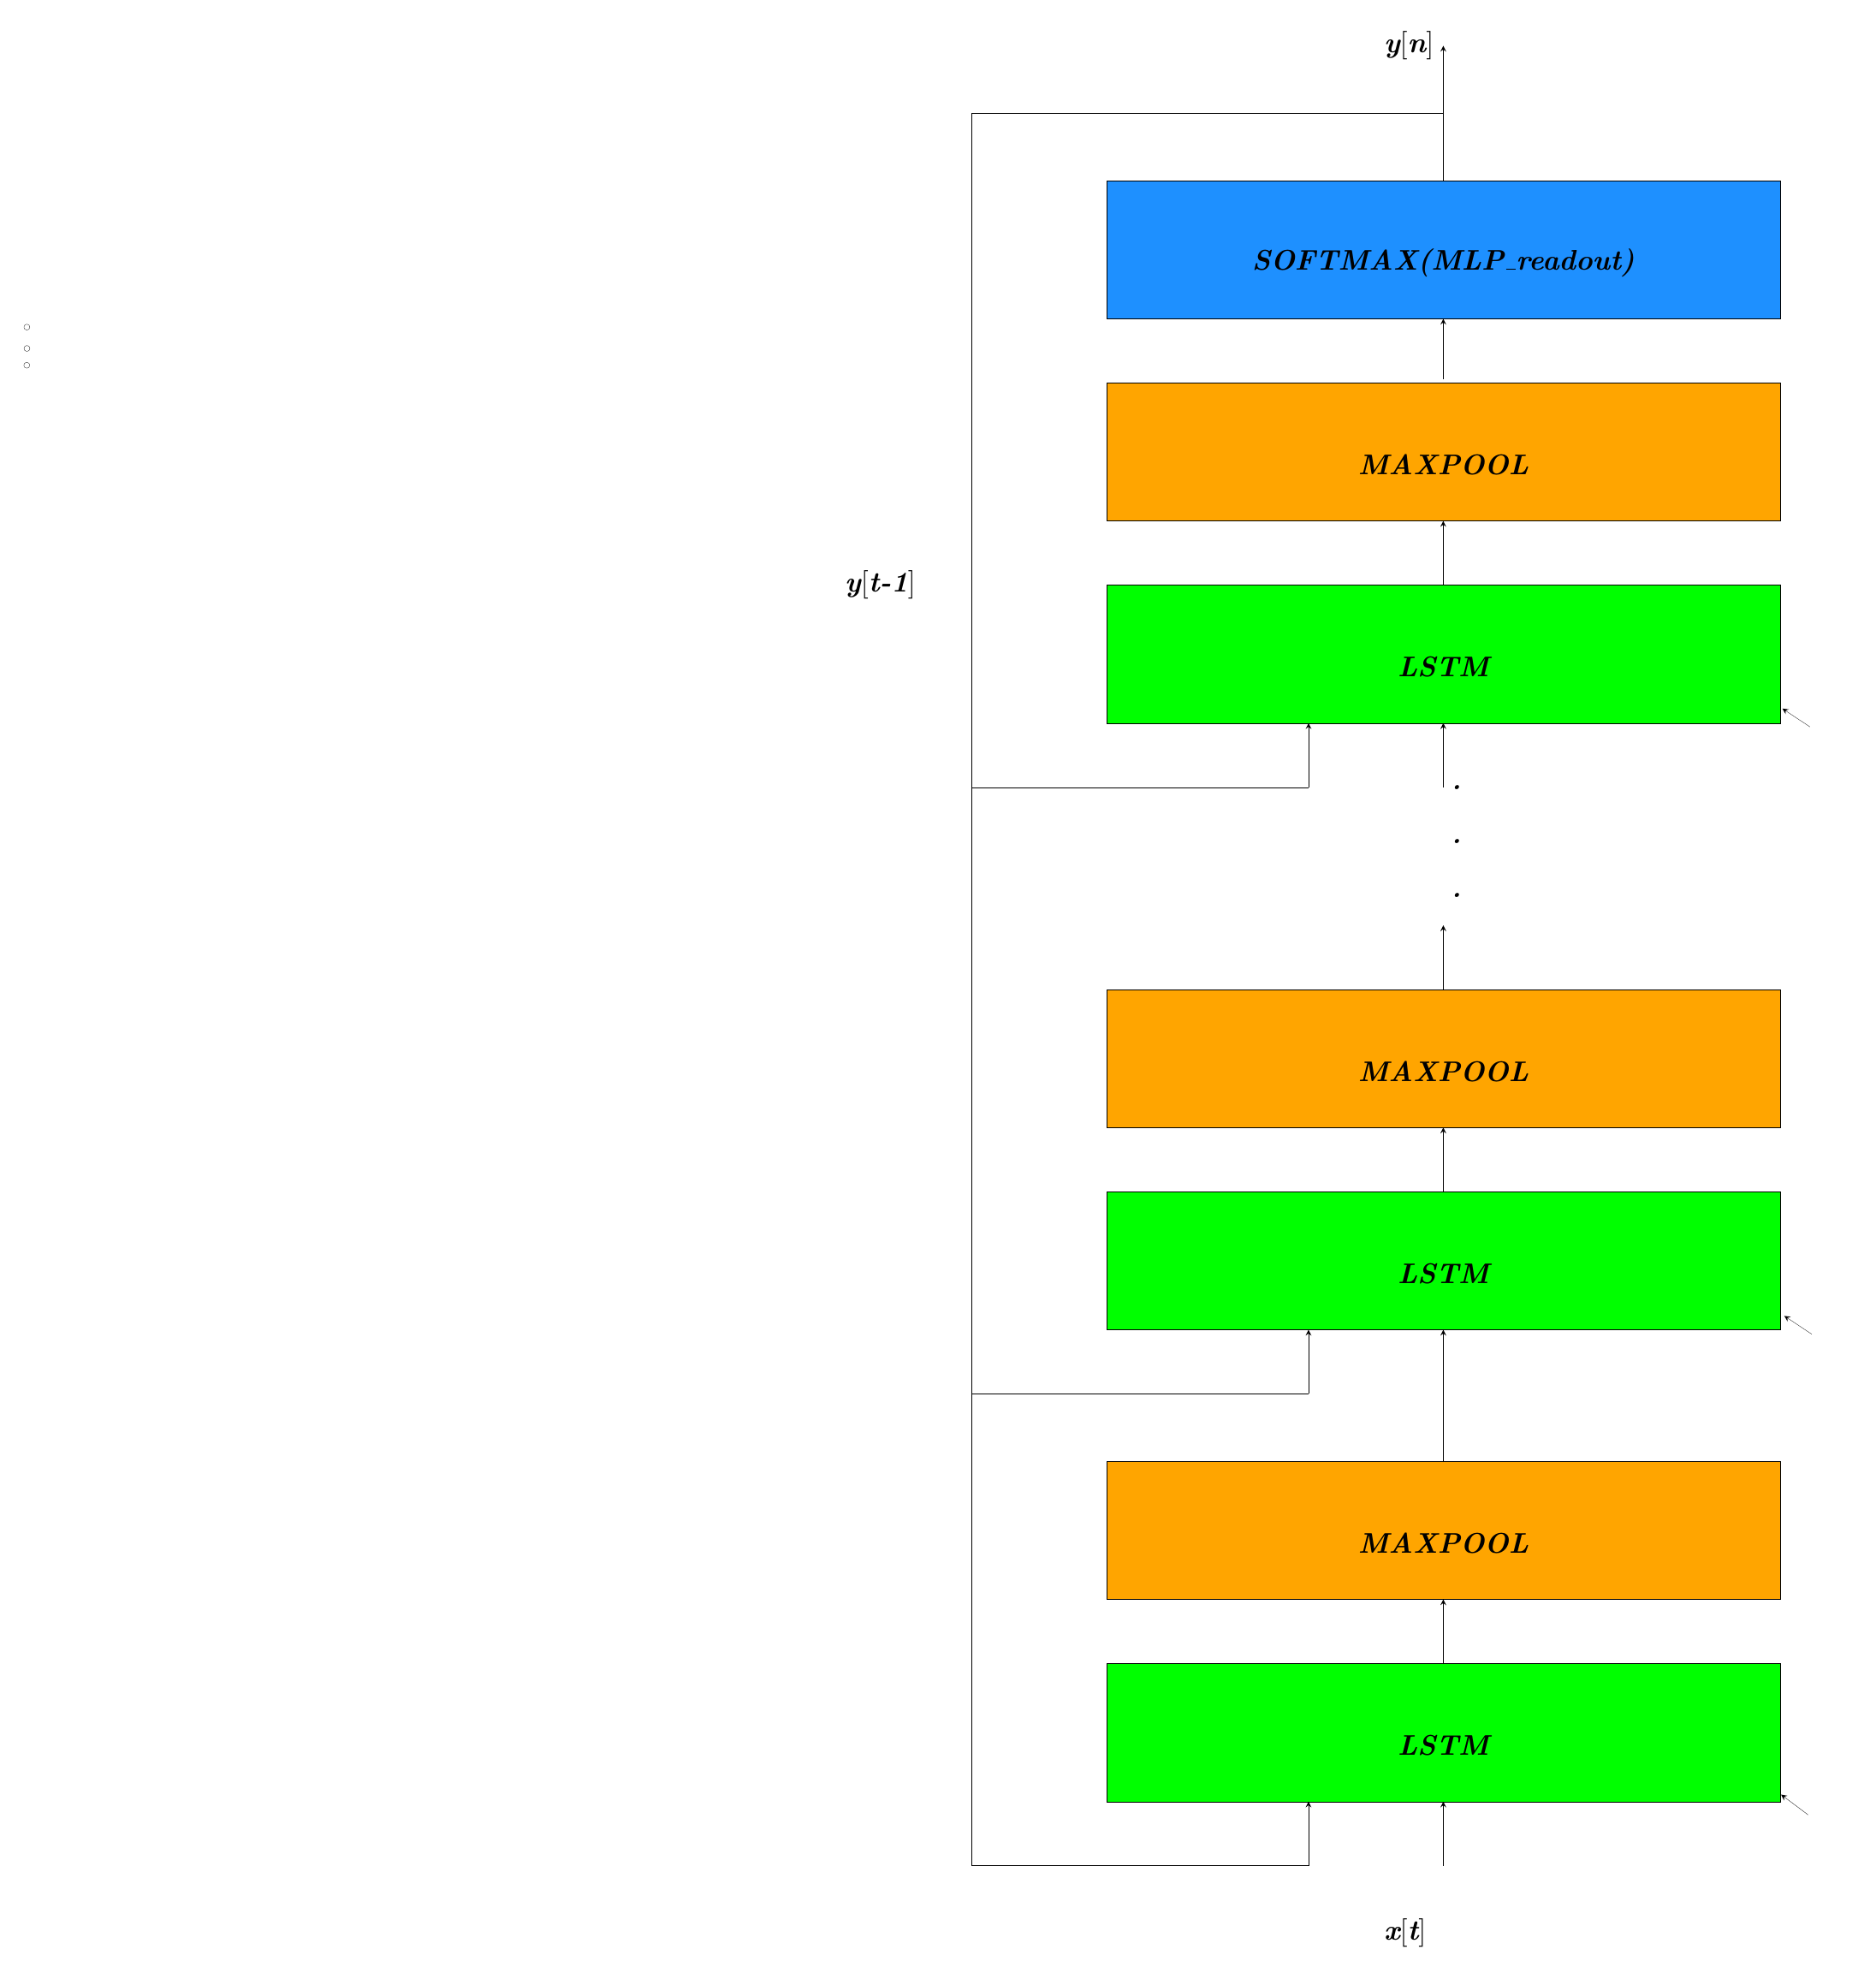
\begin{tikzpicture}
\pgftransformxscale{1.000000}
\pgftransformyscale{-1.000000}
\definecolor{dialinecolor}{rgb}{0.000000, 0.000000, 0.000000}
\pgfsetstrokecolor{dialinecolor}
\definecolor{dialinecolor}{rgb}{1.000000, 1.000000, 1.000000}
\pgfsetfillcolor{dialinecolor}
\definecolor{dialinecolor}{rgb}{1.000000, 1.000000, 1.000000}
\pgfsetfillcolor{dialinecolor}
\pgfpathellipse{\pgfpoint{27.921843\du}{4.950110\du}}{\pgfpoint{1.258243\du}{0\du}}{\pgfpoint{0\du}{1.250000\du}}
\pgfusepath{fill}
\pgfsetlinewidth{0.100000\du}
\pgfsetdash{}{0pt}
\pgfsetdash{}{0pt}
\pgfsetmiterjoin
\definecolor{dialinecolor}{rgb}{0.000000, 0.000000, 0.000000}
\pgfsetstrokecolor{dialinecolor}
\pgfpathellipse{\pgfpoint{27.921843\du}{4.950110\du}}{\pgfpoint{1.258243\du}{0\du}}{\pgfpoint{0\du}{1.250000\du}}
\pgfusepath{stroke}
% setfont left to latex
\definecolor{dialinecolor}{rgb}{0.000000, 0.000000, 0.000000}
\pgfsetstrokecolor{dialinecolor}
\node at (27.921843\du,5.145110\du){};
\definecolor{dialinecolor}{rgb}{1.000000, 1.000000, 1.000000}
\pgfsetfillcolor{dialinecolor}
\pgfpathellipse{\pgfpoint{27.949843\du}{13.960800\du}}{\pgfpoint{1.258243\du}{0\du}}{\pgfpoint{0\du}{1.250000\du}}
\pgfusepath{fill}
\pgfsetlinewidth{0.100000\du}
\pgfsetdash{}{0pt}
\pgfsetdash{}{0pt}
\pgfsetmiterjoin
\definecolor{dialinecolor}{rgb}{0.000000, 0.000000, 0.000000}
\pgfsetstrokecolor{dialinecolor}
\pgfpathellipse{\pgfpoint{27.949843\du}{13.960800\du}}{\pgfpoint{1.258243\du}{0\du}}{\pgfpoint{0\du}{1.250000\du}}
\pgfusepath{stroke}
% setfont left to latex
\definecolor{dialinecolor}{rgb}{0.000000, 0.000000, 0.000000}
\pgfsetstrokecolor{dialinecolor}
\node at (27.949843\du,14.155800\du){};
\definecolor{dialinecolor}{rgb}{1.000000, 0.647059, 0.000000}
\pgfsetfillcolor{dialinecolor}
\fill (17.000000\du,17.000000\du)--(17.000000\du,19.050000\du)--(27.000000\du,19.050000\du)--(27.000000\du,17.000000\du)--cycle;
\pgfsetlinewidth{0.100000\du}
\pgfsetdash{}{0pt}
\pgfsetdash{}{0pt}
\pgfsetmiterjoin
\definecolor{dialinecolor}{rgb}{0.000000, 0.000000, 0.000000}
\pgfsetstrokecolor{dialinecolor}
\draw (17.000000\du,17.000000\du)--(17.000000\du,19.050000\du)--(27.000000\du,19.050000\du)--(27.000000\du,17.000000\du)--cycle;
% setfont left to latex
\definecolor{dialinecolor}{rgb}{0.000000, 0.000000, 0.000000}
\pgfsetstrokecolor{dialinecolor}
\node at (22.000000\du,18.220000\du){MAXPOOL};
\definecolor{dialinecolor}{rgb}{0.000000, 1.000000, 0.000000}
\pgfsetfillcolor{dialinecolor}
\fill (17.000000\du,4.000000\du)--(17.000000\du,6.050000\du)--(27.000000\du,6.050000\du)--(27.000000\du,4.000000\du)--cycle;
\pgfsetlinewidth{0.100000\du}
\pgfsetdash{}{0pt}
\pgfsetdash{}{0pt}
\pgfsetmiterjoin
\definecolor{dialinecolor}{rgb}{0.000000, 0.000000, 0.000000}
\pgfsetstrokecolor{dialinecolor}
\draw (17.000000\du,4.000000\du)--(17.000000\du,6.050000\du)--(27.000000\du,6.050000\du)--(27.000000\du,4.000000\du)--cycle;
% setfont left to latex
\definecolor{dialinecolor}{rgb}{0.000000, 0.000000, 0.000000}
\pgfsetstrokecolor{dialinecolor}
\node at (22.000000\du,5.220000\du){LSTM};
\definecolor{dialinecolor}{rgb}{0.000000, 1.000000, 0.000000}
\pgfsetfillcolor{dialinecolor}
\fill (17.000000\du,13.000000\du)--(17.000000\du,15.050000\du)--(27.000000\du,15.050000\du)--(27.000000\du,13.000000\du)--cycle;
\pgfsetlinewidth{0.100000\du}
\pgfsetdash{}{0pt}
\pgfsetdash{}{0pt}
\pgfsetmiterjoin
\definecolor{dialinecolor}{rgb}{0.000000, 0.000000, 0.000000}
\pgfsetstrokecolor{dialinecolor}
\draw (17.000000\du,13.000000\du)--(17.000000\du,15.050000\du)--(27.000000\du,15.050000\du)--(27.000000\du,13.000000\du)--cycle;
% setfont left to latex
\definecolor{dialinecolor}{rgb}{0.000000, 0.000000, 0.000000}
\pgfsetstrokecolor{dialinecolor}
\node at (22.000000\du,14.220000\du){LSTM};
\definecolor{dialinecolor}{rgb}{1.000000, 0.647059, 0.000000}
\pgfsetfillcolor{dialinecolor}
\fill (17.000000\du,10.000000\du)--(17.000000\du,12.050000\du)--(27.000000\du,12.050000\du)--(27.000000\du,10.000000\du)--cycle;
\pgfsetlinewidth{0.100000\du}
\pgfsetdash{}{0pt}
\pgfsetdash{}{0pt}
\pgfsetmiterjoin
\definecolor{dialinecolor}{rgb}{0.000000, 0.000000, 0.000000}
\pgfsetstrokecolor{dialinecolor}
\draw (17.000000\du,10.000000\du)--(17.000000\du,12.050000\du)--(27.000000\du,12.050000\du)--(27.000000\du,10.000000\du)--cycle;
% setfont left to latex
\definecolor{dialinecolor}{rgb}{0.000000, 0.000000, 0.000000}
\pgfsetstrokecolor{dialinecolor}
\node at (22.000000\du,11.220000\du){MAXPOOL};
\definecolor{dialinecolor}{rgb}{0.117647, 0.564706, 1.000000}
\pgfsetfillcolor{dialinecolor}
\fill (17.000000\du,-2.000000\du)--(17.000000\du,0.050000\du)--(27.000000\du,0.050000\du)--(27.000000\du,-2.000000\du)--cycle;
\pgfsetlinewidth{0.100000\du}
\pgfsetdash{}{0pt}
\pgfsetdash{}{0pt}
\pgfsetmiterjoin
\definecolor{dialinecolor}{rgb}{0.000000, 0.000000, 0.000000}
\pgfsetstrokecolor{dialinecolor}
\draw (17.000000\du,-2.000000\du)--(17.000000\du,0.050000\du)--(27.000000\du,0.050000\du)--(27.000000\du,-2.000000\du)--cycle;
% setfont left to latex
\definecolor{dialinecolor}{rgb}{0.000000, 0.000000, 0.000000}
\pgfsetstrokecolor{dialinecolor}
\node at (22.000000\du,-0.780000\du){SOFTMAX(MLP\_readout)};
\pgfsetlinewidth{0.100000\du}
\pgfsetdash{}{0pt}
\pgfsetdash{}{0pt}
\pgfsetbuttcap
{
\definecolor{dialinecolor}{rgb}{0.000000, 0.000000, 0.000000}
\pgfsetfillcolor{dialinecolor}
% was here!!!
\pgfsetarrowsend{stealth}
\definecolor{dialinecolor}{rgb}{0.000000, 0.000000, 0.000000}
\pgfsetstrokecolor{dialinecolor}
\draw (22.000000\du,23.000000\du)--(22.000000\du,22.050000\du);
}
\pgfsetlinewidth{0.100000\du}
\pgfsetdash{}{0pt}
\pgfsetdash{}{0pt}
\pgfsetbuttcap
{
\definecolor{dialinecolor}{rgb}{0.000000, 0.000000, 0.000000}
\pgfsetfillcolor{dialinecolor}
% was here!!!
\pgfsetarrowsend{stealth}
\definecolor{dialinecolor}{rgb}{0.000000, 0.000000, 0.000000}
\pgfsetstrokecolor{dialinecolor}
\draw (22.000000\du,20.000000\du)--(22.000000\du,19.050000\du);
}
\pgfsetlinewidth{0.100000\du}
\pgfsetdash{}{0pt}
\pgfsetdash{}{0pt}
\pgfsetbuttcap
{
\definecolor{dialinecolor}{rgb}{0.000000, 0.000000, 0.000000}
\pgfsetfillcolor{dialinecolor}
% was here!!!
\pgfsetarrowsend{stealth}
\definecolor{dialinecolor}{rgb}{0.000000, 0.000000, 0.000000}
\pgfsetstrokecolor{dialinecolor}
\draw (22.000000\du,17.000000\du)--(22.000000\du,15.050000\du);
}
\pgfsetlinewidth{0.100000\du}
\pgfsetdash{}{0pt}
\pgfsetdash{}{0pt}
\pgfsetbuttcap
{
\definecolor{dialinecolor}{rgb}{0.000000, 0.000000, 0.000000}
\pgfsetfillcolor{dialinecolor}
% was here!!!
\pgfsetarrowsend{stealth}
\definecolor{dialinecolor}{rgb}{0.000000, 0.000000, 0.000000}
\pgfsetstrokecolor{dialinecolor}
\draw (22.000000\du,13.000000\du)--(22.000000\du,12.050000\du);
}
% setfont left to latex
\definecolor{dialinecolor}{rgb}{0.000000, 0.000000, 0.000000}
\pgfsetstrokecolor{dialinecolor}
\node[anchor=west] at (21.000000\du,5.000000\du){};
% setfont left to latex
\definecolor{dialinecolor}{rgb}{0.000000, 0.000000, 0.000000}
\pgfsetstrokecolor{dialinecolor}
\node[anchor=west] at (22.000000\du,7.000000\du){.};
% setfont left to latex
\definecolor{dialinecolor}{rgb}{0.000000, 0.000000, 0.000000}
\pgfsetstrokecolor{dialinecolor}
\node[anchor=west] at (22.000000\du,7.800000\du){.};
% setfont left to latex
\definecolor{dialinecolor}{rgb}{0.000000, 0.000000, 0.000000}
\pgfsetstrokecolor{dialinecolor}
\node[anchor=west] at (22.000000\du,8.600000\du){.};
\pgfsetlinewidth{0.100000\du}
\pgfsetdash{}{0pt}
\pgfsetdash{}{0pt}
\pgfsetbuttcap
{
\definecolor{dialinecolor}{rgb}{0.000000, 0.000000, 0.000000}
\pgfsetfillcolor{dialinecolor}
% was here!!!
\pgfsetarrowsend{stealth}
\definecolor{dialinecolor}{rgb}{0.000000, 0.000000, 0.000000}
\pgfsetstrokecolor{dialinecolor}
\draw (22.000000\du,10.000000\du)--(22.000000\du,9.050000\du);
}
\pgfsetlinewidth{0.100000\du}
\pgfsetdash{}{0pt}
\pgfsetdash{}{0pt}
\pgfsetbuttcap
{
\definecolor{dialinecolor}{rgb}{0.000000, 0.000000, 0.000000}
\pgfsetfillcolor{dialinecolor}
% was here!!!
\pgfsetarrowsend{stealth}
\definecolor{dialinecolor}{rgb}{0.000000, 0.000000, 0.000000}
\pgfsetstrokecolor{dialinecolor}
\draw (22.000000\du,7.000000\du)--(22.000000\du,6.050000\du);
}
\pgfsetlinewidth{0.100000\du}
\pgfsetdash{}{0pt}
\pgfsetdash{}{0pt}
\pgfsetbuttcap
{
\definecolor{dialinecolor}{rgb}{0.000000, 0.000000, 0.000000}
\pgfsetfillcolor{dialinecolor}
% was here!!!
\pgfsetarrowsend{stealth}
\definecolor{dialinecolor}{rgb}{0.000000, 0.000000, 0.000000}
\pgfsetstrokecolor{dialinecolor}
\draw (22.000000\du,4.000000\du)--(22.000000\du,3.050000\du);
}
\definecolor{dialinecolor}{rgb}{1.000000, 1.000000, 1.000000}
\pgfsetfillcolor{dialinecolor}
\pgfpathellipse{\pgfpoint{27.883243\du}{21.050000\du}}{\pgfpoint{1.258243\du}{0\du}}{\pgfpoint{0\du}{1.250000\du}}
\pgfusepath{fill}
\pgfsetlinewidth{0.100000\du}
\pgfsetdash{}{0pt}
\pgfsetdash{}{0pt}
\pgfsetmiterjoin
\definecolor{dialinecolor}{rgb}{0.000000, 0.000000, 0.000000}
\pgfsetstrokecolor{dialinecolor}
\pgfpathellipse{\pgfpoint{27.883243\du}{21.050000\du}}{\pgfpoint{1.258243\du}{0\du}}{\pgfpoint{0\du}{1.250000\du}}
\pgfusepath{stroke}
% setfont left to latex
\definecolor{dialinecolor}{rgb}{0.000000, 0.000000, 0.000000}
\pgfsetstrokecolor{dialinecolor}
\node at (27.883243\du,21.245000\du){};
\definecolor{dialinecolor}{rgb}{0.000000, 1.000000, 0.000000}
\pgfsetfillcolor{dialinecolor}
\fill (17.000000\du,20.000000\du)--(17.000000\du,22.050000\du)--(27.000000\du,22.050000\du)--(27.000000\du,20.000000\du)--cycle;
\pgfsetlinewidth{0.100000\du}
\pgfsetdash{}{0pt}
\pgfsetdash{}{0pt}
\pgfsetmiterjoin
\definecolor{dialinecolor}{rgb}{0.000000, 0.000000, 0.000000}
\pgfsetstrokecolor{dialinecolor}
\draw (17.000000\du,20.000000\du)--(17.000000\du,22.050000\du)--(27.000000\du,22.050000\du)--(27.000000\du,20.000000\du)--cycle;
% setfont left to latex
\definecolor{dialinecolor}{rgb}{0.000000, 0.000000, 0.000000}
\pgfsetstrokecolor{dialinecolor}
\node at (22.000000\du,21.220000\du){LSTM};
\pgfsetlinewidth{0.100000\du}
\pgfsetdash{}{0pt}
\pgfsetdash{}{0pt}
\pgfsetbuttcap
{
\definecolor{dialinecolor}{rgb}{0.000000, 0.000000, 0.000000}
\pgfsetfillcolor{dialinecolor}
% was here!!!
\pgfsetarrowsend{stealth}
\definecolor{dialinecolor}{rgb}{0.000000, 0.000000, 0.000000}
\pgfsetstrokecolor{dialinecolor}
\draw (27.412200\du,22.246200\du)--(27.012200\du,21.946200\du);
}
\pgfsetlinewidth{0.100000\du}
\pgfsetdash{}{0pt}
\pgfsetdash{}{0pt}
\pgfsetbuttcap
{
\definecolor{dialinecolor}{rgb}{0.000000, 0.000000, 0.000000}
\pgfsetfillcolor{dialinecolor}
% was here!!!
\pgfsetarrowsend{stealth}
\definecolor{dialinecolor}{rgb}{0.000000, 0.000000, 0.000000}
\pgfsetstrokecolor{dialinecolor}
\draw (27.468300\du,15.115600\du)--(27.060100\du,14.844700\du);
}
\pgfsetlinewidth{0.100000\du}
\pgfsetdash{}{0pt}
\pgfsetdash{}{0pt}
\pgfsetbuttcap
{
\definecolor{dialinecolor}{rgb}{0.000000, 0.000000, 0.000000}
\pgfsetfillcolor{dialinecolor}
% was here!!!
\pgfsetarrowsend{stealth}
\definecolor{dialinecolor}{rgb}{0.000000, 0.000000, 0.000000}
\pgfsetstrokecolor{dialinecolor}
\draw (27.440300\du,6.104960\du)--(27.032100\du,5.833990\du);
}
\definecolor{dialinecolor}{rgb}{1.000000, 0.647059, 0.000000}
\pgfsetfillcolor{dialinecolor}
\fill (17.000000\du,1.000000\du)--(17.000000\du,3.050000\du)--(27.000000\du,3.050000\du)--(27.000000\du,1.000000\du)--cycle;
\pgfsetlinewidth{0.100000\du}
\pgfsetdash{}{0pt}
\pgfsetdash{}{0pt}
\pgfsetmiterjoin
\definecolor{dialinecolor}{rgb}{0.000000, 0.000000, 0.000000}
\pgfsetstrokecolor{dialinecolor}
\draw (17.000000\du,1.000000\du)--(17.000000\du,3.050000\du)--(27.000000\du,3.050000\du)--(27.000000\du,1.000000\du)--cycle;
% setfont left to latex
\definecolor{dialinecolor}{rgb}{0.000000, 0.000000, 0.000000}
\pgfsetstrokecolor{dialinecolor}
\node at (22.000000\du,2.220000\du){MAXPOOL};
\pgfsetlinewidth{0.100000\du}
\pgfsetdash{}{0pt}
\pgfsetdash{}{0pt}
\pgfsetbuttcap
{
\definecolor{dialinecolor}{rgb}{0.000000, 0.000000, 0.000000}
\pgfsetfillcolor{dialinecolor}
% was here!!!
\pgfsetarrowsend{stealth}
\definecolor{dialinecolor}{rgb}{0.000000, 0.000000, 0.000000}
\pgfsetstrokecolor{dialinecolor}
\draw (22.000000\du,0.950226\du)--(22.000000\du,0.050000\du);
}
\pgfsetlinewidth{0.100000\du}
\pgfsetdash{}{0pt}
\pgfsetdash{}{0pt}
\pgfsetbuttcap
{
\definecolor{dialinecolor}{rgb}{0.000000, 0.000000, 0.000000}
\pgfsetfillcolor{dialinecolor}
% was here!!!
\pgfsetarrowsend{stealth}
\definecolor{dialinecolor}{rgb}{0.000000, 0.000000, 0.000000}
\pgfsetstrokecolor{dialinecolor}
\draw (22.000000\du,-2.000000\du)--(22.000000\du,-4.000000\du);
}
% setfont left to latex
\definecolor{dialinecolor}{rgb}{0.000000, 0.000000, 0.000000}
\pgfsetstrokecolor{dialinecolor}
\node[anchor=west] at (21.000000\du,24.000000\du){x\ensuremath{[}t\ensuremath{]}};
% setfont left to latex
\definecolor{dialinecolor}{rgb}{0.000000, 0.000000, 0.000000}
\pgfsetstrokecolor{dialinecolor}
\node[anchor=west] at (21.000000\du,-4.000000\du){y\ensuremath{[}n\ensuremath{]}};
\pgfsetlinewidth{0.100000\du}
\pgfsetdash{}{0pt}
\pgfsetdash{}{0pt}
\pgfsetbuttcap
{
\definecolor{dialinecolor}{rgb}{0.000000, 0.000000, 0.000000}
\pgfsetfillcolor{dialinecolor}
% was here!!!
\definecolor{dialinecolor}{rgb}{0.000000, 0.000000, 0.000000}
\pgfsetstrokecolor{dialinecolor}
\draw (20.000000\du,23.000000\du)--(15.000000\du,23.000000\du);
}
\pgfsetlinewidth{0.100000\du}
\pgfsetdash{}{0pt}
\pgfsetdash{}{0pt}
\pgfsetbuttcap
{
\definecolor{dialinecolor}{rgb}{0.000000, 0.000000, 0.000000}
\pgfsetfillcolor{dialinecolor}
% was here!!!
\pgfsetarrowsend{stealth}
\definecolor{dialinecolor}{rgb}{0.000000, 0.000000, 0.000000}
\pgfsetstrokecolor{dialinecolor}
\draw (20.000000\du,16.000000\du)--(20.000000\du,15.050000\du);
}
\pgfsetlinewidth{0.100000\du}
\pgfsetdash{}{0pt}
\pgfsetdash{}{0pt}
\pgfsetbuttcap
{
\definecolor{dialinecolor}{rgb}{0.000000, 0.000000, 0.000000}
\pgfsetfillcolor{dialinecolor}
% was here!!!
\definecolor{dialinecolor}{rgb}{0.000000, 0.000000, 0.000000}
\pgfsetstrokecolor{dialinecolor}
\draw (20.000000\du,16.000000\du)--(15.000000\du,16.000000\du);
}
\pgfsetlinewidth{0.100000\du}
\pgfsetdash{}{0pt}
\pgfsetdash{}{0pt}
\pgfsetbuttcap
{
\definecolor{dialinecolor}{rgb}{0.000000, 0.000000, 0.000000}
\pgfsetfillcolor{dialinecolor}
% was here!!!
\pgfsetarrowsend{stealth}
\definecolor{dialinecolor}{rgb}{0.000000, 0.000000, 0.000000}
\pgfsetstrokecolor{dialinecolor}
\draw (20.000000\du,7.000000\du)--(20.000000\du,6.050000\du);
}
\pgfsetlinewidth{0.100000\du}
\pgfsetdash{}{0pt}
\pgfsetdash{}{0pt}
\pgfsetbuttcap
{
\definecolor{dialinecolor}{rgb}{0.000000, 0.000000, 0.000000}
\pgfsetfillcolor{dialinecolor}
% was here!!!
\definecolor{dialinecolor}{rgb}{0.000000, 0.000000, 0.000000}
\pgfsetstrokecolor{dialinecolor}
\draw (20.000000\du,7.000000\du)--(15.000000\du,7.000000\du);
}
% setfont left to latex
\definecolor{dialinecolor}{rgb}{0.000000, 0.000000, 0.000000}
\pgfsetstrokecolor{dialinecolor}
\node[anchor=west] at (13.000000\du,4.000000\du){y\ensuremath{[}t-1\ensuremath{]}};
\pgfsetlinewidth{0.100000\du}
\pgfsetdash{}{0pt}
\pgfsetdash{}{0pt}
\pgfsetbuttcap
{
\definecolor{dialinecolor}{rgb}{0.000000, 0.000000, 0.000000}
\pgfsetfillcolor{dialinecolor}
% was here!!!
\definecolor{dialinecolor}{rgb}{0.000000, 0.000000, 0.000000}
\pgfsetstrokecolor{dialinecolor}
\draw (22.000000\du,-3.000000\du)--(15.000000\du,-3.000000\du);
}
\pgfsetlinewidth{0.100000\du}
\pgfsetdash{}{0pt}
\pgfsetdash{}{0pt}
\pgfsetbuttcap
{
\definecolor{dialinecolor}{rgb}{0.000000, 0.000000, 0.000000}
\pgfsetfillcolor{dialinecolor}
% was here!!!
\definecolor{dialinecolor}{rgb}{0.000000, 0.000000, 0.000000}
\pgfsetstrokecolor{dialinecolor}
\draw (15.000000\du,-3.000000\du)--(15.000000\du,6.000000\du);
}
\pgfsetlinewidth{0.100000\du}
\pgfsetdash{}{0pt}
\pgfsetdash{}{0pt}
\pgfsetbuttcap
{
\definecolor{dialinecolor}{rgb}{0.000000, 0.000000, 0.000000}
\pgfsetfillcolor{dialinecolor}
% was here!!!
\definecolor{dialinecolor}{rgb}{0.000000, 0.000000, 0.000000}
\pgfsetstrokecolor{dialinecolor}
\draw (15.000000\du,3.000000\du)--(15.000000\du,23.000000\du);
}
\pgfsetlinewidth{0.100000\du}
\pgfsetdash{}{0pt}
\pgfsetdash{}{0pt}
\pgfsetbuttcap
{
\definecolor{dialinecolor}{rgb}{0.000000, 0.000000, 0.000000}
\pgfsetfillcolor{dialinecolor}
% was here!!!
\pgfsetarrowsend{stealth}
\definecolor{dialinecolor}{rgb}{0.000000, 0.000000, 0.000000}
\pgfsetstrokecolor{dialinecolor}
\draw (20.000000\du,23.000000\du)--(20.000000\du,22.050000\du);
}
\end{tikzpicture}
} %
    \caption {
      The entire structure of the sequence homogeneously-structured classifier
      (SHC).
      \label{fig:shc_diagram}
    }
    %\end{center}
\end{figure}

Fig. \ref{fig:shc_diagram} shows the structure of the SHC algorithm. The
structure is very simple and somewhat similar to that of CTC shown in TODO


\subsection{Training of the Sequence Homogeneously-Structured Classifier}
In this section, we describe how to train SHC. The procedure is summarized
in the following table.

\section{Structure of the Recurrent Sequence Recognizer}
\subsection{Review of the Room Simulator for Data Augmentation}
%
%
\begin{figure}
  \centering
    \begin{subfigure}{\linewidth}
      \centering
      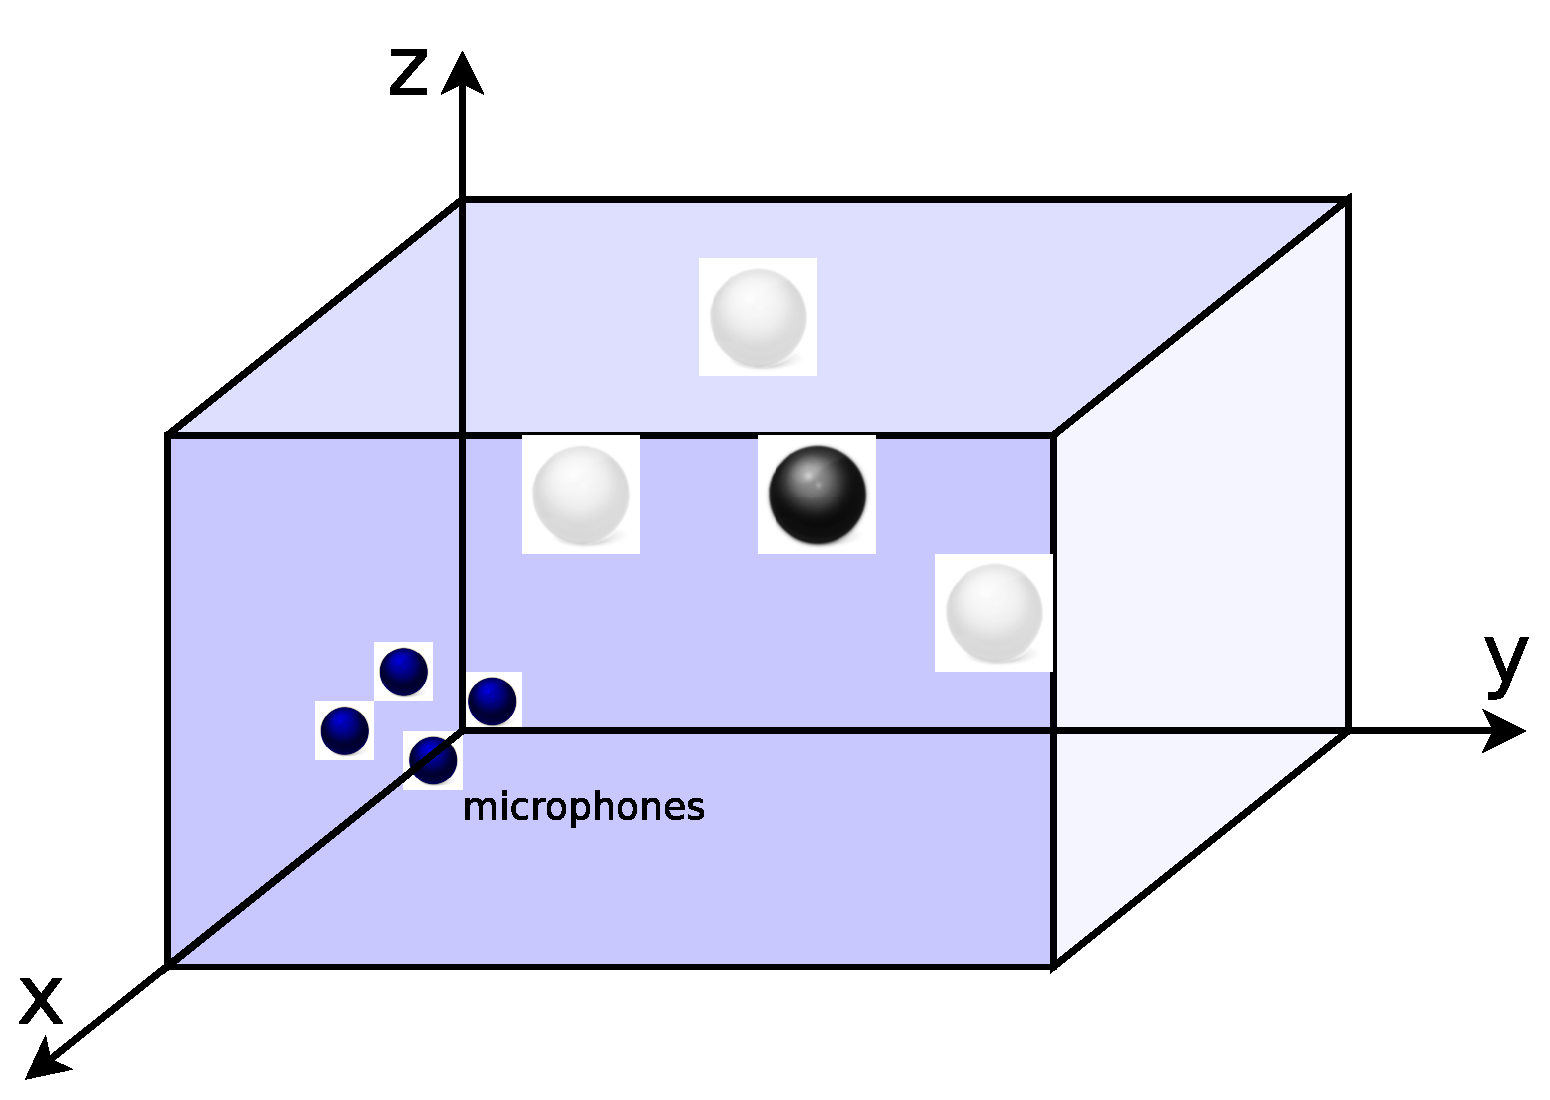
\includegraphics[width=70mm]{room_diagram.eps}
      \caption{}
      \label{fig:room_diagram}
    \end{subfigure}
   \\
    \begin{subfigure}{\linewidth}
      \centering
      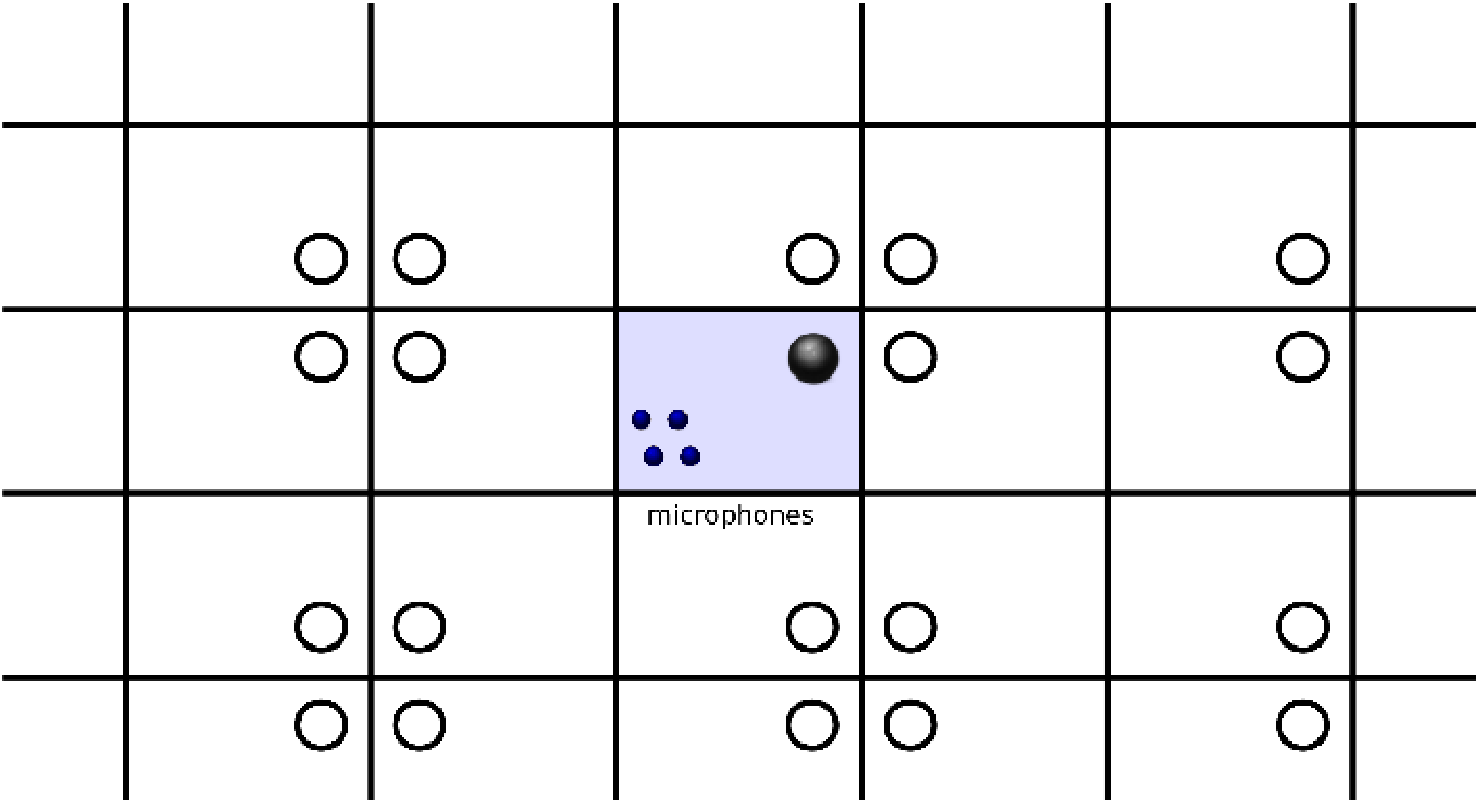
\includegraphics[width=70mm]{image_method.eps}
      \caption{}
      \label{fig:image_method}
    \end{subfigure}
    \caption{
    (a) A simulated room: There may be multiple microphones, a single target
    sound source, multiple noise sources in a cuboid-shape room with
    acoustically reflective walls. (b) A diagram showing the location
    of the real and the virtual sound sources assuming that the walls
    reflects acoustic wave like a mirror \cite{C_Kim_INTERSPEECH_2017_1}.}
  \vspace{-10mm}
\end{figure}
%
%
%
\subsection{Viterbi alignment and N-best alignment}

In conventional frame-wise CE-training, forced-alignment 
has been performed to obtain the frame-level acoustic unit  
boundaries. TODO(chanwcom) Even though the Viterbi algorithm
has advantages in simplicity and efficiency, it is based on
the conditional independence assumption.


\subsection{Feature extraction}

Even though the log-mel coefficients have been widely used
as features for speech recognition \cite{sbdavisandpm1980},
the log non-linearity has a disadvantage in that the value
diverges to negative infinity as the mel filterbank coefficient
approaches zero \cite{C_Kim_IEEETran_2016_1}.
Thus, we use the power-law nonlinearity
rather than the log-nonlinearity:
\begin{align}
  q[m, l] =  (p[m, l])^{\frac{1}{15}}
  \label{eq:power_law_nonlineartiy}
\end{align}
We use the power coefficient of $\frac{1}{15}$ as in
\cite{C_Kim_IEEETran_2016_1, C_Kim_ICASSP_2012_1}.



In this section, we discuss how to predict the clean feature and the
error ratio from the corrupt feature. Let us denote the clean target feature,
the corrupt feature by $\boldsymbol{x}, \boldsymbol{y}$ respectively.

Using the room simulation system described in \cite{C_Kim_INTERSPEECH_2017_1},
we create a pair of clean and
corrupt utterances. Log-mel [XX] features are calculated from these original clean
and corrupt utterances. Let us denote the clean feature by $\boldsymbol{t}_i$ and
the simulated corrupt feature by $\boldsymbol{x}_i$, respectively where $i$ is the
utterance index. The training set is represented by the following set:
\begin{align}
  \mathcal{T} = \{<\boldsymbol{x}_i, \boldsymbol{t}_i>| 0 \le i \le N - 1\}
\end{align}
where $N$ is the number of training examples.

In the ECE algorithm, we first estimate the true target $\boldsymbol{t}_i$. The
estimation error is defined by the following equation:
\begin{align}
  \boldsymbol{e}_i =  \boldsymbol{t}_i - \boldsymbol{x}_i, \quad 0 \le i \le N - 1
\end{align}

The norm of the error vector $\boldsymbol{e}_i$ would be generally large when
the norm of the estimated clean feature is large.

Thus, instead of trying to estimate the error itself, the neural network tries to
estimate the error ratio given as follows:

\begin{align}
  r_i = {}{}
\end{align}

\section{Generation of simulated clean and noisy data sets}
\label{gen_inst}

To train neural networks described in section \ref{sec:estimation}, we
need a training set consisting of pairs of clean speech and noisy speech.
Unfortunately, it is not easy to have such a training set from real speech
utterances. Thus, we use the simulation system described in
\cite{C_Kim_INTERSPEECH_2017_1} to synthetically generate noisy speech
utterances from the clean speech utterances.

In our application, for clean training set, we used Wall Street Journal (WSJ)
si-284. For noise set, we used the Resource Management 1 (RM1)
\cite{price_p_ldc_1993} 50 \% of time 
and DEMAND noise [TODO(chanwcom) Adds reference] for the remaining 50 \% of time.

TODO(chanwcom) Cite DEMAND noise set.





%
%
%
%\begin{figure*}
%  \centering
%    \begin{subfigure}[\label{fig:randomly_selected_grid_coordinates}]{0.5\textwidth} {
%        \includegraphics[width=\textwidth]{target_estimation}}
%    \caption{Grid from random-sampling}
%    \end{subfigure}
%   % \begin{subfigure}[\label{fig:intersection_point}]{0.5\textwidth} {
%   %   \includegraphics[width=\textwidth]{intersection_point}}
%   % \caption{Calculation of grid coordinates}
%   % \end{subfigure}
%  \caption {Random Grid Sampling}
%\end{figure*}
%
%
%
\section{Estimation of the optimal weight in the EFW algorithm}
In this section, we describe the procedure of feature weighting approach.
Suppose that the feature before enhancement is represented by $\vec{x}$.
Let us represent the inference neural network to estimate the target by
$\mathcal{T}$.

\begin{align}
  \mathcal{X} = \{  \}
\end{align}

Instead of directly using the enhanced feature $\widehat{\vec{y}}$, we consider
the following interpolated feature $\bm{z}$ from the original corrupt
input $\bm{x}$ and .
\begin{align}
  \vec{z} = \vec{w} \odot \widehat{\vec{y}} \ + (1 - \vec{w}) \odot \vec{x} 
    \label{eq:vec_z}
\end{align}
where $\odot$ denotes the Hadamard product (entry-wise product).

Let us denote the estimated variance vector by $\hat{\vec{v}}$:
\begin{align}
  \hat{\vec{v}} & = \text{Var}[\widehat{\vec{y}}] \nonumber \\
                & = E[(y - y)^2 | \vec{x}[0], \vec{x}[1], ... \vec{x}[T]]
     \label{eq:vec_v}
\end{align}

In our discussion, let us assume that the expectation of $\hat{\vec{y}}$ is the
same as the true target $\vec{y}$.
\begin{align}
  E[\widehat{\vec{y}}] = \vec{y}  \label{eq:expectation_of_y}
\end{align}

Now, let us obtain the expected value of $\vec{z}$ from
\eqref{eq:vec_z} and \eqref{eq:expectation_of_y}
\begin{align}
  E[\vec{z}] = (1 - \vec{w}) \odot (\vec{x} - \vec{y})
\end{align}
Thus, the bias of $\vec{z}$ is given by:
\begin{align}
  Bias_{\vec{z}} & = E[\vec{z}] - t \nonumber \\
                 & = \vec{w} \odot (\widehat{\vec{y}} - \vec{y})
\end{align}

From \eqref{eq:vec_z} and \eqref{eq:vec_v}, the variance of $\vec{z}$ is given by:
\begin{align}
  Var_{\vec{z}} = \vec{v} \odot w \odot w.
\end{align}
The mean squared error of the $i$-th element of the $\vec{z}$ is given by:
\begin{align}
  MSE_{\vec{z_i}} & = Bias_{\vec{z_i}}^2 + Var_{\vec{z_i}} \nonumber \\
                 & =  \left[(\vec{x}_i - \vec{y}_i) ^ 2
                    + \vec{v}_i^2 \right] \vec{w}_i^{2}
                    - 2 (\vec{x}_i - \vec{y}_i)^{2}  \vec{w}_i
                    + (\vec{x}_i - \vec{y}_i)^{2}
 \label{eq:mse_z_i}
\end{align}
Since the above equation \eqref{eq:mse_z_i} is a quadratic equation with
respect to $\vec{w}_i$, we may find that the minimum value of $MSE_{\vec{z_i}}$
is obtained when $\vec{w}_i$ has the following value:
\begin{align}
  \vec{w}_i = \frac{(\vec{x}_i - \vec{y}_i)^2}{(\vec{x}_i - \vec{y}_i)^2 + \vec{v}_i}
\end{align}

Thus, the final form of the estimated vector $\widehat{\vec{z}}$ becomes:
\begin{align}
  \widehat{\vec{z}} = \widehat{\vec{w}} \odot \widehat{\vec{y}}
    \ + (1 - \widehat{\vec{w}}) \odot \vec{x}
\end{align}
where
\begin{align}
  \widehat{\vec{w}} = {(\vec{x} - \vec{y})^{\odot 2}}
    \left[(\vec{x} - \vec{y})^{\odot 2}+ \vec{v}\right]^{\odot -1}.
\end{align}


Sequence enhancement

The feature enhancement is to map a sequence of corrupt features $\mathbf{X}$.
\begin{subequations}
  \begin{align}
    \mathbf{X} = \left(\vec{x}[0], \vec{x}[1], \cdots, \vec{x}[M-1] \right)  \\
    \mathbf{Y} = \left(\vec{y}[0], \vec{y}[1], \cdots, \vec{y}[M-1] \right) 
  \end{align}
\end{subequations}

\subsubsection*{Acknowledgments}

\section*{References}

References follow the acknowledgments. Use unnumbered first-level
heading for the references. Any choice of citation style is acceptable
as long as you are consistent. It is permissible to reduce the font
size to \verb+small+ (9 point) when listing the references. {\bf
  Remember that you can go over 8 pages as long as the subsequent ones contain
  \emph{only} cited references.}
\medskip

\small

\clearpage
\newpage
\bibliographystyle{plain}
\bibliography{../../common_bib_file/common_bib_file}



\end{document}
